% 数値計算 理論面

\section{はじめに}
数値計算とは,代数的または解析的に解くことが難しい,もしくは計算量が膨大になってしまうような問題を,コンピューターを用いて計算する手法のこと.
数値計算は
本稿では、この数値計算という手法の基礎を解説する.

\section{数値計算とシミュレーション}
コンピューターシミュレーション,という言葉を聞いたことがあるだろうか.
津波が都市のどこまで被害を及ぼすかや,天体の形成のシミュレーション,というのは聞いたことがあるかもしれない.

\begin{figure}[htbp]
	\begin{minipage}[t]{0.45\hsize}
        \centering
        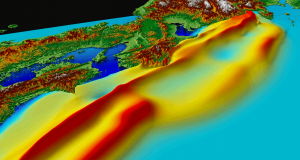
\includegraphics[width=5cm]{img/jamstec-kei-tsunami.png}
        \subcaption{海洋研究開発機構の津波シミュレーション}
    \end{minipage}
	\begin{minipage}[t]{0.45\hsize}
        \centering
    	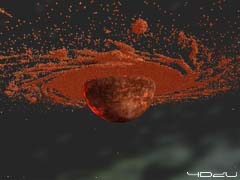
\includegraphics[width=5cm]{img/4d2u-giant-impact.jpg}
    	\subcaption{国立天文台の月形成シミュレーション}
    \end{minipage}
    \caption{コンピュータシミュレーションの例}
\end{figure}

このように,実際に実験を行うことが不可能であるような問題を研究するにあたって,コンピューターシミュレーションは現在では必要不可欠な技術となっている.

では,こうした物理現象をコンピューターシミュレーションを使って再現するには,どのようなことが必要なのかというと,具体的には\ref{numerical-analysis-flow}のような手順を踏む.

\begin{figure}
	\centering
    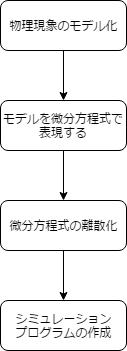
\includegraphics[width=2.5cm]{img/numerical-analysis-flow.png}
    \caption{コンピューターシミュレーションの手順}
    \label{numerical-analysis-flow}
\end{figure}


まずは,シミュレーションする物理現象をモデル化する.
モデル化とは,現実の問題から必要な部分だけを取り出し,問題を単純化することだ.
例えば,手に持ったボールを静かに離して落下させたとしよう.
このとき,実際の物理現象としては,ボールは
手についた汗で滑ったり,
空気抵抗によって減速されたり,
回転していたり
と,様々なことが起きており,これらは全てボールの運動に影響を及ぼす.
しかし,これらによるボールの運動への影響はとても小さいため,「ボールの落下運動」を考えるにあたっては,無視しても問題はない.
これも一種のモデル化である.
さて,これで問題をモデル化することは出来たので,次にこのモデルを微分方程式で表現しよう.

\section{微分方程式と物理現象}
そもそも,微分方程式とは何かというと,簡単に言えば微分形を含む方程式のことだ.
例えば,
\begin{align}
	\dfrac{dx}{dt} = x
\end{align}
などがある.

\subsection{微分の復習}
ここで,微分とはなんだったかを軽く復習しよう.
\subsubsection{平均変化率}
まずは,直線の傾きのことを考えてみよう.
ある直線を表す関数$y=f(x)$があるとして,この傾きを求めようと思ったら,どのようにすればいいだろうか.

\begin{figure}[h]
	\centering
	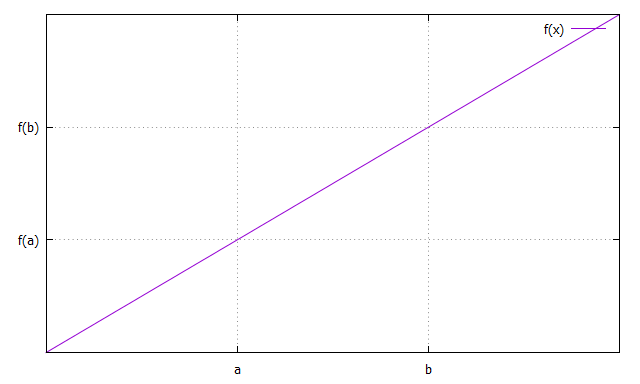
\includegraphics[width=5.5cm]{img/average-rate-of-change.png}
    \caption{$f(x)$の平均変化率}
\end{figure}

答えは簡単で,$f(x)$の変化量を$x$の変化量で割ればいい.
傾きを$\alpha $とおくと,
\begin{align}
	\alpha = \dfrac{f(b)-f(a)}{b-a}
    \label{average-rate-of-change}
\end{align}
となる.
このような傾き$\alpha$のことを,$f(x)$の$x$が$a$から$b$まで変化するときの平均変化率という.

\subsubsection{平均変化率の極限}
さて,直線の関数の平均変化率はすべての区間において同じなので,今度は曲線の関数の平均変化率について考えてみよう.
曲線を表す関数$f(x)$があるとして,先程と同じように,$x$が$a$から$b$まで変化するときの平均変化率を考える.
曲線の平均変化率を考えるときは,点$(a,f(a))$と点$(b,f(b))$を結ぶ直線$l$を考え,この直線$l$について,直線の平均変化率を求めればよい.
\begin{figure}[htbp]
	\centering
	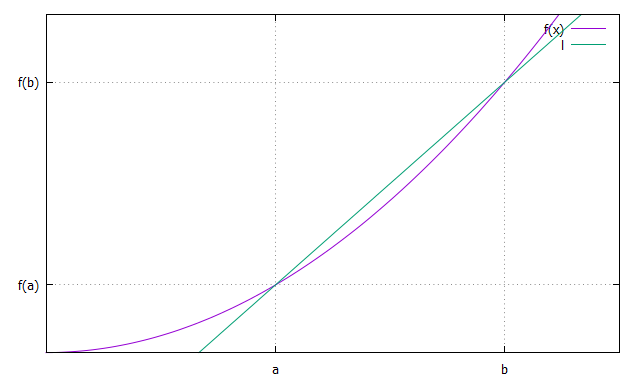
\includegraphics[width=5cm]{img/curve-average-rate-of-change.png}
    \caption{曲線の平均変化率}
    \label{curve-average-rate-of-change}

\end{figure}
そのため,平均変化率$\alpha$を求める式は\ref{average-rate-of-change}と全く同じである.

これで曲線においても平均変化率を求めることが出来たわけだが,図\ref{curve-average-rate-of-change}を見れば分かるように,あくまでこれは「平均の変化率」であり,$b-a$の値が大きければ大きくなるほど,直線$l$は曲線とはかけ離れていき,平均変化率は曲線の変化率とはなかなか言いにくくなってくる.

\subsubsection{微分係数}
そのため,今度は$b-a$の値をどんどん小さくしてしまえばどうだろうか,というのが微分の第一歩である.
$b-a$の値をどんどん小さくするというのは,「$b$を限りなく$a$に近づける」ということに等しい.
このように,ある値を別のある値に"限りなく近づける"ということを,「極限」といい,
\begin{align}
b \to a
\end{align}

のように書く.
さて,今考えたいのは$b \to a$のときの平均変化率$\alpha$であった.
極限を表す記号である$\lim{}$を使って平均変化率を求める式\ref{curve-average-rate-of-change}を書き直すと,\ref{limit-rate-of-change}のようになる.

\begin{align}
\lim_{b \to a} \dfrac{f(b)-f(a)}{b-a}
\label{limit-rate-of-change}
\end{align}

しかし,このままでは少し分かりにくいので,$b-a = h$とおいて書き直すと\ref{limit-rate-of-change-2}

\begin{align}
\alpha = \lim_{h \to 0} \dfrac{f(a+h)-f(a)}{h}
\label{limit-rate-of-change-2}
\end{align}

のようになる.
こうなると、$\alpha$はもはや「平均の」変化率などではなく、「瞬間の」変化率と言えるだろう.
このような、「瞬間の」変化率のことを数学的には「$x=a$における微分係数」という.

$x=a$における微分係数は$f'(a)$と表す.

よって微分係数$f'(a)$の定義は\ref{differential-coefficient-definition}のようになる.
\begin{align}
f'(a) = \lim_{h \to 0} \dfrac{f(a+h)-f(a)}{h}
\label{differential-coefficient-definition}
\end{align}

\newpage
\subsubsection{導関数}
前項で、$f(x)$の$x=a$における微分係数$f'(a)$を定義したわけだが,この$a$というのはある特定の$x$の値であった.
これを特定の値$a$ではなく,変数$x$にあてはめると,$f'(x)$という新たな関数が導かれる.
この「導かれた関数」のことを「導関数」といい,ある関数$f(x)$からその導関数$f'(x)
$を求めることを,「微分する」という.

\begin{align}
f'(x) = \lim_{h \to 0} \dfrac{f(x+h)-f(x)}{h}
\label{lagrange-notation}
\end{align}

ちなみに,これは正確には関数$f(x)$を「xについて」微分するという操作だが,何の変数で微分するかを明確に示したい場合には,導関数を\ref{leibniz-notation}のように表すこともある.
\footnote{\ref{lagrange-notation}をラグランジュ記法,\ref{leibniz-notation}をライプニッツ記法という.}

\begin{align}
\dfrac{d}{dx} f(x)
\label{leibniz-notation}
\end{align}


%ある関数$f(x)$があったときに,$x=x,x+\Delta x$
%(ここで、$\Delta x$は微小量)
%での$f(x)$の値$f(x),f(x+\Delta x)$

\section{オイラー法}
微分について簡単に復習したところで,数値計算の話に戻ろう.

数値計算の手法には様々なものがあるが,その中でも,最も簡単な手法の一つであるオイラー法は,先ほど復習した微分の定義から簡単に導くことができる.
導関数の定義を再掲すると,
\begin{align}
f'(x) = \lim_{h \to 0} \dfrac{f(x+h)-f(x)}{h}
\end{align}
であった.
ここで,$h \to 0$としているが,コンピューターではこのような極限値は扱えない\footnote{後述する}ため,$h$を「限りなく0に近づける」のではなく,「そこそこ」0に近い値をhとすることで,$f'(x)$を近似することができる.
これは,「平均変化率」と同じ考え方である.
\begin{align}
f'(x) \approx \dfrac{f(x+h)-f(x)}{h}
\label{numerical-differentiation}
\end{align}

式\ref{numerical differentiation}より,$f(x)$が既知であれば,$h$をある程度小さい値として同式に代入すると,$f'(x)$に近い値,つまり近似値を得る事ができる.

では実際に,式\ref{numerical differentiation}を使って導関数を近似してみよう.


$f(x)=x^2$とすると,導関数$f'(x)$の「正しい値」は$f'(x)=2x$である.
このように,解析的に答えが分かっているとき,これを解析解という(これとは逆に,数値計算によって求めた解のことを数値解という).
では,$h=0.01$として計算し,数値解と解析解の値を比べてみよう.
\begin{figure}

\label{numerical-differentiation-graph}
\end{figure}

図\ref{numerical differentiation-graph}より,数値解と解析解は大体重なっており,ある程度の精度で数値解が解析解を近似できていることが分かる.
このように,数値的に導関数の値を求める,つまり微分を行うことができたわけだが,式\ref{numerical-differentiation}を変形すると,\ref{euler-method-definition}のようになる.

\begin{eqnarray}
f(x+h)-f(x) &\approx& h f'(x) \\
f(x+h) &\approx& f(x) + h f'(x)
\label{euler-method-definition}
\end{eqnarray}

式\ref{euler-method-definition}より,$f(x)$が未定義でも,どこかの$f(x)$の値と導関数$f'(x)$,hが分かっていれば,$f(x+h)$の近似値を求めることができる,ということが分かる.

これにより何ができるかというと,$f'(x),h,f(a)$が既知とすると,
\begin{eqnarray}
f(a+h)  &\approx& f(a) + h f'(a) \\
f(a+2h) &\approx& f(a+h) + h f'(a+h) \\
f(a+3h) &\approx& f(a+2h) + h f'(a+2h) \\
...
\end{eqnarray}
というように,$h$ごとに「飛び飛び」に$f(x)$の値を次々に近似していくことができる.
このように,既知の$f'(x)$を用いて$f(x)$の値を求める(近似)ことを,「数値積分」という.

この場合は,$f(a)$の値が最初に必要なので,この$f(a)$のことを初期値といい,また,「飛び飛び」の度合いである$h$のことをステップ幅もしくは刻み幅という.


先程とおなじように,数値積分を実際にやってみよう.


$f'(x)=2x$とすると,解析解は$f(x)=\int f'(x) dx = x^2 + C$($C$は積分定数)となる.
ここで,初期値を$f(0)=0$とすると,$f(x)$に代入して,
\begin{eqnarray}
f(0) = 0 + C = 0 \\
\therefore C = 0
\end{eqnarray}
より積分定数が定まり,$f(x) = x^2$.


$h=0.01$として,これらを数値積分し,数値解と解析解を重ねてみると,図\ref{euler-method-graph}のようになる.

\begin{figure}
\label{euler-method-graph}
\end{figure}

ここでも,数値解はある程度の精度で解析解を近似していることが分かる.

このようにして数値積分を行う手法のことを,数学者レオンハルト・オイラー
\footnote{18世紀の数学の中心となり,続く19世紀の厳密化・抽象化時代の礎を築いた.彼の名を冠した定理はたくさんある.}
の名を冠して,オイラー法
\footnote{正確には,これは前進オイラー法というもので,これの他に陰解法である後進オイラー法や,修正オイラー法というものがある.}
という.

\section{ルンゲクッタ法}
ごめんなさい,時間がなくなってしまいました.

\section{参考文献}
https://www.esrij.com/industries/case-studies/55425/
http://4d2u.nao.ac.jp
http://www.ele.kanagawa-it.ac.jp/~takeo/sk/NumericalComputation.pdf
